% Source program: module_perturbjtw2009.sas
% Last updated:

\begin{figure}[th]
\caption{Sensitivity Analysis}
%\begin{subfigure}
\begin{tabular}{ccc}
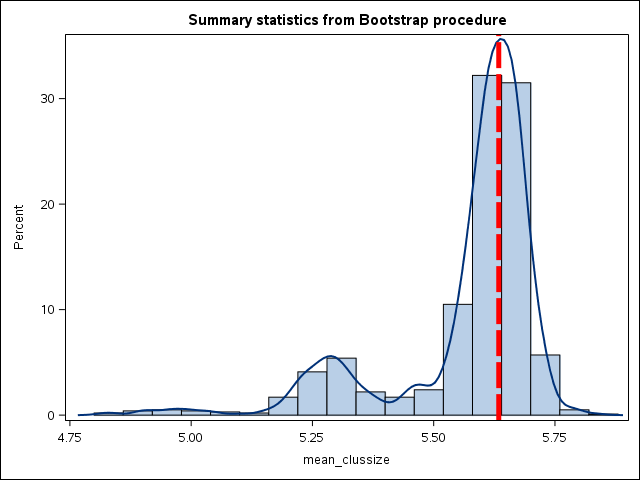
\includegraphics[width=0.33\textwidth]{./figures/mean_clussize_jtw2009.png}
&
%\caption{Mean Cluster Size}
%\end{subfigure}
%\begin{subfigure}
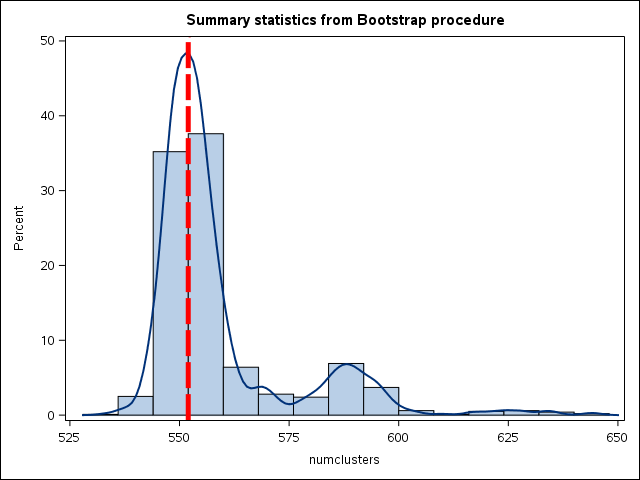
\includegraphics[width=0.33\textwidth]{./figures/numclusters_jtw2009.png}
&
%\caption{Number of Clusters}
%\end{subfigure}
%\begin{subfigure}
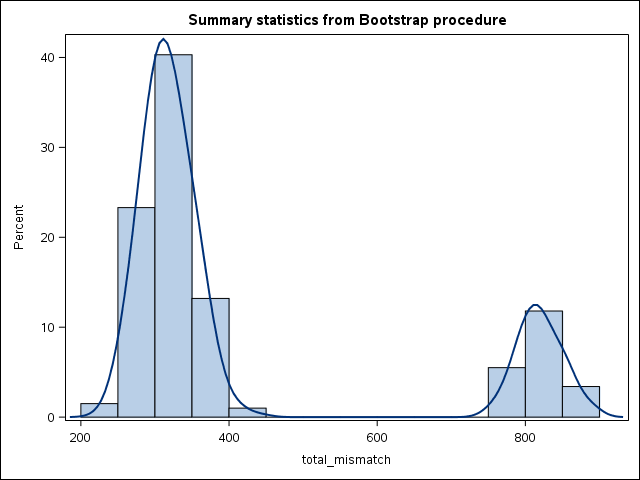
\includegraphics[width=0.33\textwidth]{./figures/mismatchedcounties_jtw2009.png}
\\
{(a) Mean Cluster Size}&
{(b) Number of Clusters}&
%\caption
{(c)Mismatched Counties}
\\
\multicolumn{3}{p{6.2in}}{\footnotesize \emph{Notes:} Histograms plot the density of summary statistics from commuting zones produced using the TS1996 methodology from 1000 simulations of Margins of Error from the 2009-2013 ACS commuting flows data. Red lines provide the summary statistics from commuting zones produced from the published ACS estimates (mean cluster size of 5.63 for 552 clusters).}\\
%\end{subfigure}
\end{tabular}
\label{fig:perturbation}
\end{figure}
\normalsize 

